\documentclass{report}
\usepackage[utf8]{inputenc}
\usepackage[italian]{babel}
\usepackage{titling}
\usepackage[style=ieee]{biblatex}
\usepackage{hyperref}
\usepackage{textcomp}
\usepackage{tabularx}
\usepackage{graphicx}
\usepackage{listings}
\usepackage{comment}
\usepackage{nameref}
\usepackage{float}
\usepackage{wrapfig}
\hypersetup{
    colorlinks,
    citecolor=black,
    filecolor=black,
    linkcolor=black,
    urlcolor=black
}

\addbibresource{108456-masini.bib}
\graphicspath{ {./imgs/} }
\lstset{
  basicstyle=\small,
  breaklines=true
}

\newcommand{\srsnomeprogetto}{GPMS}
\newcommand{\srslongnomeprogetto}{General Purpose Monitoring System}

\title{
    \srsnomeprogetto\linebreak
    \large \textit \srslongnomeprogetto \linebreak
    \large Specifica dei requisiti di progetto}
\author{Gabriele Masini \#108456}
\date{2019-12-10 rev.2020-02-10}

\begin{document}
    
\maketitle
\pagenumbering{gobble}
\newpage
\tableofcontents
\newpage
\pagenumbering{arabic}

\chapter{Introduzione}
La disciplina denominata \textit{DSP}, dall'inglese \textit{Digital Signal Processing} ovvero ``elaborazione digitale di segnali'', è stata ed è tuttora parte fondamentale dello sviluppo tecnologico digitale che caratterizza la storia dell'umanità a partire dalla seconda metà del ventesimo secolo. Ciò è dovuto al fatto che gran parte delle grandezze di interesse scentifico e ingegneristico che debbono essere analizzate ed elaborate hanno natura di segnali, i quali necessitano di particolari accortezze e algoritmi per essere elaborati da un dispositivo a capacità di calcolo e memoria limitate, come il calcolatore elettronico.

L'elaborazione digitale dei segnali interessa particolarmente il campo delle telecomunicazioni, dove si lotta per ottenere bitrate sempre maggiori su lunghissime distanze. Un esempio lampante sono le linee telefoniche: dai commutatori analogici, costosi e poco pratici, si è passati ai canali digitali, che a parità di qualità audio offrono un maggior numero di connessioni contemporanee sullo stesso supporto (il doppino telefonico), non necessitano di interruttori analogici e soprattutto hanno un costo sia in termini di costruzione sia di messa in operazione e manutenzione nettamente minore.

Non bisogna però restringere il proprio campo visivo alle sole telecomunicazioni, poiché le tecnologie DSP vengono largamente utilizzate anche in altri campi e risultano fondamentali per applicazioni come video e audio processing, applicazioni mediche, militari, finanziarie e di ricerca.

\section{Scopo}
La presente tesi si pone come obbiettivo quello di studiare e implementare alcuni dei tanti algoritmi che vengono utilizzati nell'ambito DSP sia dal punto di vista essenzialmente sequenziale del processore, sia una loro possibile parallelizzazione su scheda grafica. Ciò non significa che gli algoritmi riportati siano nella loro forma più efficiente o performante, bensì sono mostrati in modo da far risaltare le differenze implementative che espongono sulle due piattaforme. Inoltre gli algoritmi vengono realizzati con un minimo utilizzo di librerie esterne, in quanto è nell'interesse della tesi e dell'autore l'approfondimento degli algoritmi stessi e lo studio del loro funzionamento interno.

Per portare a termine tale scopo è stata necessaria la stesura di un programma in grado di eseguire gli algoritmi studiati e implementati sia su CPU sia su GPU. Si è deciso di limitarsi all'elaborazione di file audio a canale singolo poiché oltre ad ottenere un riscontro in termini di forma d'onda e spettri di frequenza e fase è possibile anche verificarne il funzionamento in base all'effetto che si ottiene nell'ascolto del risultato. Il programma, con le dovute modifiche, si può estendere anche all'elaborazione di segnali diversi dall'audio.

\section{Inquadramento}
Il presente elaborato espone nel capitolo \ref{cap:nozioni} alcune nozioni matematiche necessarie per la corretta comprensione e spiegazione delle implementazioni degli algoritmi presentati in seguito. Viene spiegato, inoltre, come si utilizza la GPU dal punto di vista implementativo, quali sono i ``componenti di calcolo'' principali e come vi si interfaccia con le API di CUDA.

Nel capitolo \ref{cap:implementazione} vengono presentate e spiegate le parti più interessanti degli algoritmi studiati, i quali sono interamente disponibili nel repository GitHub della tesi \cite{repo}.

\chapter{Nozioni prerequisite}
Prima di cimentarsi in implementazioni di algoritmi è assolutamente necessario comprenderne la loro natura matematica. A tale scopo vengono presentate brevemente in questa sezione alcune nozioni fondamentali per l'elaborazione di segnali digitali.

\section{Concetti fondamentali in DSP}
\subsection{Segnali, sistemi lineari}
Nel corso di questa tesi verranno presentati spesso i termini \textit{segnale} e \textit{sistema} per cui è necessario definirli. Un segnale è ``una descrizione di come un parametro varia rispetto ad un altro parametro''\cite{dspguide}. Esempi di segnali sono: pressione dell'aria nel tempo (audio), coppia motrice rispetto al numero di giri di un motore etc.

Per studiare i segnali e modificarne l'andamento si fa riferimento ai sistemi. Un sistema è ``un qualsiasi processo che produce un segnale in uscita in risposta ad un segnale in ingresso''\cite{dspguide}. In particolare si studiano i sistemi lineari, ovvero sistemi che seguono le proprietà necessarie per la linearità algebrica (omogeneità e additività). La proprietà di linearità è fondamentale nel DSP perché permette di scomporre il problema in sottoproblemi più piccoli e facilmente risolvibili per poi ricombinarli assieme e ottenere il risultato del problema di partenza.

\subsection{Convoluzione}
Il primo strumento fondamentale per comprendere gli algoritmi DSP è l'operazione di convoluzione tra segnali. Essa è definita nel seguente modo\cite{calandrino}:
\begin{equation}
    x(t) * y(t) = \int_{-\infty}^{+\infty}x(\tau)y(t-\tau)d\tau
\end{equation}
Dove $x$ e $y$ sono i due segnali da convolvere.

La convoluzione per segnali discreti è definita da una sommatoria\cite{dspguide}:
\begin{equation}
    y[k] = \displaystyle\sum_{j=0}^{M-1}h[j]x[i-j]
\end{equation}
Dove $x$ e $h$ sono i segnali da convolvere, $y$ il risultato della loro convoluzione. $M$ è il numero di punti del segnale $h$. È fondamentale precisare che il segnale risultante dalla convoluzione discreta di $x$ e $h$ contiene $N+M-1$ punti, dove $N$ indica il numero di punti del segnale $x$.


\subsection{La trasformata di fourier}
Strumento essenziale per gli algoritmi DSP, la trasformata di Fourier scompone un segnale nel dominio del tempo nelle sue componenti nel dominio delle frequenze. Esistono trasformate diverse per diversi tipi di rappresentazione dei segnali nel tempo e una classificazione accettata a livello matematico e ingegneristico\cite{dspguide} è la seguente:

\begin{center}
\begin{small}
\begin{tabular}{p{0.4\linewidth} p{0.4\linewidth}}
    Tipo segnale & Trasformata utilizzata \\
    \hline
    Aperiodico tempo-continuo & Trasformata di fourier continua (CFT) \\
    Periodico tempo-continuo & Serie di fourier \\
    Aperiodico tempo-discreto & Trasformata di fourier tempo discreta (DTFT) \\
    Periodico tempo-discreto & Trasformata di fourier discreta (DFT)
\end{tabular}
\end{small}
\end{center}

\medskip

Le formule (trasformazione e antitrasformazione) della CFT sono definite nel modo seguente\cite{calandrino}:
\begin{equation}
    {F}(\omega) = \int_{-\infty}^{+\infty} f(t){e}^{-j \omega t} dt
\end{equation}
\begin{equation}
    {f}(t) = \frac{1}{2\pi}\int_{-\infty}^{+\infty} F(\omega){e}^{+j \omega t} d\omega
\end{equation}
Dove $f(t)$ identifica il segnale nel dominio dei tempi, $F(\omega)$ la sua trasformata e $j$ è l'unità immaginaria tale che $j^2 = -1$.

La serie di fourier invece è definita come\cite{calandrino}:
\begin{equation}
    {f}(t) = \displaystyle\sum_{n=-\infty}^{+\infty} c_n e^{jn \omega_0 t} \quad, \quad \omega_0 = \frac{2\pi}{T}
\end{equation}
con
\begin{equation}
    c_n = \frac{1}{T}\int_{-\frac{T}{2}}^{+\frac{T}{2}}f(t)e^{-jn \omega_0 t} dt
\end{equation}
Dove $T$ è il periodo della funzione e $c_n$ è il coefficiente $n$-esimo della serie. Gli spettri di ampiezza e di fase si ricavano dai valori di $A_n$ e $\varphi_n$ definiti nel seguente modo:
\begin{equation}
    c_0 = A_0
\end{equation}
\begin{equation}
    2 c_n = A_n e^{-j\varphi_n} \quad,\quad n \geq 1
\end{equation}
Essi generano degli spettri a righe in corrispondenza delle pulsazioni multiple di $\omega_0$.

Per quanto la CFT e la serie di Fourier siano degli strumenti matematici indispensabili per comprendere l'analisi dei segnali, esse trovano relativamente poca applicazione pratica nella elaborazione dei segnali, poiché solitamente i segnali che devono essere processati da un calcolatore hanno natura tempo-discreta (ovvero sono stati campionati) e necessitano, quindi, dell'utilizzo della DTFT o della DFT. Come vedremo in seguito, però, si utilizza sempre la DFT, in quanto non è possibile modellare in un calcolatore il concetto di ``infinito'' fondamentale per la definizione e il calcolo della DTFT\cite{dspguide}.

\subsection{La trasformata di Fourier Discreta (DFT)}
Come presentato nella sezione precedente, la DFT trasforma un segnale tempo-discreto periodico nelle sue componenti nel dominio delle frequenze; essa per un segnale di $N$ punti è definita nel seguente modo\cite{dspguide}:
\begin{equation}
    X[k] = \frac{1}{N}\displaystyle\sum_{n=0}^{N-1}x[n]e^{-j 2\pi kn/N}
\end{equation}
Si presti attenzione al fatto che la trasformata è definita su $N$ punti da $0$ a $N-1$ ed essi rappresentano le frequenze positive per $0 \leq n \leq N/2$ e frequenze negative per $N/2 \leq n \leq N-1$, poiché lo spettro di frequenze di un segnale discreto è periodico. Questo comporta che la trasformata di un segnale reale abbia la parte reale dello spettro in simmetria pari rispetto a $N/2$ e parte immaginaria in simmetria dispari rispetto a $N/2$.

L'operazione di antitrasformazione è definita nel modo seguente:
\begin{equation}
    x[n] = \displaystyle\sum_{k=0}^{N-1}X[k]e^{j 2\pi kn/N}
\end{equation}

\section{GPU e CUDA}
Lo studio delle implementazioni su GP-GPU viene effettuato tramite l'utilizzo della tecnologia CUDA proprietaria di Nvidia. Essa espone una interfaccia di programmazione per l'utilizzo del calcolo parallelo delle schede grafiche di proprietà di Nvidia in linguaggio di programmazione C++.

È vantaggioso studiare implementazioni su schede video in quanto esse permettono di effettuare un elevato numero di operazioni parallele su un certo insieme di dati; infatti il termine scheda ``video'' deriva dal fatto che in principio erano utilizzate soprattutto per l'elaborazione e rendering di video, dove sono necessarie elaborazioni simili per tanti dati quanti sono i pixel dell'immagine. In tempi relativamente recenti, però, si è smesso di parlare di GPU come schede video, ma si parla di GP-GPU acronimo di \textit{General Purpose Graphical Processing Unit}, ovvero ``Schede video per scopi generici'', poiché hanno trovato largo utilizzo per quanto riguarda elaborazioni ad alte prestazioni, soprattutto nell'ambito di ricerca di intelligenze artificiali come le reti neurali.

\subsection{Programmazione in CUDA}
Facendo riferimento alla guida per la programmazione in CUDA di Nvidia\cite{cuda_programming_guide} il principale elemento di calcolo che viene somministrato alla GPU è il \textit{kernel}, il quale è una funzione che viene eseguita un numero definito di volte in parallelo sulla GPU quando essa viene invocata. Un kernel viene dichiarato utilizzando il modificatore \lstinline{__global__}. Inoltre è importante tenere a mente che al kernel possono essere passati solo tipi predefiniti, puntatori o struct di tipi predefiniti o puntatori, a patto che i puntatori facciano riferimento ad un'area di memoria sulla GPU, non nella RAM. Questo comporta che i dati da elaborare vadano prima copiati dalla memoria centrale alla memoria della GPU, elaborati e poi ricopiati nella RAM. Le API di CUDA mettono a disposizione le funzioni necessarie per operare questi spostamenti di memoria.

I kernel possono essere raggruppati in \textit{stream} (flussi). I kernel facenti parte dello stesso stream vengono eseguiti in successione, ma stream diversi possono essere eseguiti in parallelo. Non c'è modo di sapere in quale istante un kernel entrerà in esecuzione e nemmeno quando esso finirà, per tale motivo risulta necessario porre attenzione alla sincronizzazione dei dati su cui operano i diversi kernel. Anche in questo caso le API fornite da Nvidia mettono a disposizione varie funzioni di sincronizzazione sia all'interno dei kernel di uno stesso blocco (tramite \lstinline!__syncthreads()!), sia per stream (con \lstinline!cudaStreamSynchronize(<stream>)!) sia per la GPU intera (con \lstinline!cudaDeviceSynchronize()!).

Le unità di elaborazione all'interno della GPU sono divise in blocchi ciascuno dei quali è composto da un numero di thread. Compito del programmatore è distribuire queste risorse ai kernel necessari. I blocchi e i thread al loro interno sono organizzati secondo una matrice 3-dimensionale, e i loro indici sono accessibili all'interno del kernel usando le variabili \lstinline{threadIdx} e \lstinline{blockIdx}.

Un esempio mostrato nella guida alla programmazione di Nvidia è il seguente, il quale esegue la somma di elementi di due vettori:

\begin{lstlisting}
    // Kernel definition
    __global__ void VecAdd(float* A, float* B, float* C)
    {
        int i = threadIdx.x;
        C[i] = A[i] + B[i];
    }

    int main()
    {
        ...
        // Kernel invocation with N threads
        VecAdd<<<1, N>>>(A, B, C);
        ...
    }
\end{lstlisting}

\chapter{Implementazione}

\section{Breve descrizione del programma}
Per lo studio di quanto descritto fino ad ora si è costruito un programma in grado di caricare un file \lstinline{.wav} in buffer di dimensione arbitraria in memoria per poterne elaborare il contenuto; dopodiché è possibile specificare una catena di operazioni da effettuare sul segnale e un metodo di salvataggio del risultato (\lstinline{.wav} o \lstinline{.csv}). La catena di operazioni e il salvataggio vengono specificati in un file di testo. Per la lettura e scrittura su file .wav si utilizza la libreria ``libsndfile'' scritta da Erik de Castro Lopo \cite{libsndfile}.

L'invocazione del programma avviene tramite riga di comando ed è necessario utilizzare un programma esterno per visualizzare il contenuto dei file di output. I grafici dei risultati che verranno mostrati in questa tesi sono stati generati utilizzando un file \lstinline{.csv} in uscita dal programma il quale viene poi visualizzato tramite il programma Veusz \cite{veusz}.

\section{Strutture dati utilizzate}

Per la rappresentazione dei dati dei campioni in ingressi si utilizza una struttura nominata \lstinline{SignalBuffer_t} definita nel seguente modo:

\begin{lstlisting}
struct SignalBuffer_t
{
	cuComplex* samples;
	size_t channels;
	size_t* channel_size;
	size_t max_size;
};
\end{lstlisting}

Essa continene un array di campioni, il numero di canali, la lunghezza dei buffer di ogni canale e la lunghezza massima disponibile dell'array. I campioni sono organizzati nell'array di numeri complessi secondo lo schema descritto in figura \ref{fig:signalbuffersamples}, ovvero lo stesso modo in cui vengono restituiti i dati dalle funzioni di lettura di \lstinline{libsdnfile}.

\begin{figure}[h]
    \centering
    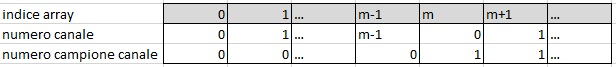
\includegraphics[width=1\textwidth]{signalbuffersamples}
    \caption{Disposizione dei campioni nella struttura \lstinline{SignalBuffer_t} supponendo $m$ canali.}
    \label{fig:signalbuffersamples}
\end{figure}

\lstinline{cuComplex} è un tipo importato dalla libreria di CUDA il quale rappresenta un numero complesso. Esso può essere utilizzato, con le apposite operazioni, sia dalla CPU sia dalla GPU.

Vengono definite anche operazioni su questa struttura, le quali garantiscono la corretta gestione dei campioni all'interno della stessa. Le funzioni utilizzate sono dichiarate con i modificatori \lstinline{__host__ __device__} i quali sono necessari al compilatore di CUDA per segnalare che tali funzioni possono essere sia eseguite sulla CPU (host), sia sulla scheda grafica (device).

\section{Convoluzione}
Il primo algoritmo che è stato studiato e implementato è la convoluzione tra segnali la quale è indispensabile perché è il primo strumento con cui si può calcolare la risposta di un sistema ad un determinato segnale se si conosce la risposta impulsiva del sistema stesso.

La definizione di convoluzione tra segnali discreti è descritta dall'equazione \ref{eq:convoluzionediscreta}. Bisogna porre particolare attenzione al fatto che la lunghezza del risultato della convoluzione è uguale alla somma delle lunghezze dei segnali in ingresso meno uno; questo comporta che bisogna far attenzione a gestire il fenomeno detto ``overlap'' tra buffer risultanti consecutivi; questo fenomeno, grazie alla linearità del sistema, si riduce solamente alla somma della ``coda'' del buffer in uscita precedente con i primi campioni del buffer in uscita seguente.

Visto che la convoluzione è una operazione che necessita di due segnali in entrata, si è supposto che il secondo segnale sia di un solo canale e non sia diviso in vari buffer, ma sia tutto contenuto in uno solo, mentre il primo segnale può essere diviso in più buffer. Questa decisione è giustificata dal fatto che spesso la convoluzione viene utilizzata tra un segnale molto lungo e uno di gran lunga più corto, poiché, come già detto, è una operazione onerosa in termini di calcolo. In particolare è spesso utilizzata per operazioni di filtraggio e in questo caso il secondo segnale prende il nome di ``kernel del filtro'' \cite[p.~108]{dspguide}. Nelle spiegazioni seguenti si utilizzerà la parola ``kernel'' per indicare il secondo segnale della convoluzione; bisogna prestare attenzione a non confondere il ``kernel'' del filtro con le funzioni ``kernel'' di CUDA.

\subsection{CPU}

La convoluzione sulla CPU è implementata utilizzando due cicli \lstinline{for}: uno che scorre i campioni del buffer in entrata di un determinato canale e l'altro invece che scorre i campioni del buffer contenente il secondo segnale. I due campioni ottenuti vengono quindi moltiplicati assieme e vengono poi aggiunti al valore di un buffer temporaneo. La presenza del buffer temporaneo è necessaria per la corretta gestione del fenomeno dell'``overlap''; il buffer temporaneo alla fine della convoluzione conterrà i campioni in uscita dalla convoluzione e la ``coda'' da sommare alla convoluzione successiva.

Una versione semplificata alle componenti fondamentali del codice che è stato utilizzato è il seguente:
\begin{lstlisting}
...
for (size_t i = 0; i < input_size; i++)
{
    cuComplex in_sample = get_sample(input, channel, i);
    for (size_t j = 0; j < kernel_size; j++)
    {
        size_t index = i+j;
        cuComplex kernel_sample = get_sample(kernel, SIGNAL_CHANNEL, j);
        cuComplex out_sample = get_sample(temp, channel, index);
        cuComplex result = cuCaddf(out_sample, cuCmulf(in_sample, kernel_sample));
        set_sample(temp, channel, index, result);
    }
}
...
\end{lstlisting}
Come si può osservare sono presenti i due cicli \lstinline{for} e le operazioni per effettuare l'accumulazione nel buffer temporaneo. Le funzioni \lstinline{cuCaddf} e \lstinline{cuCmulf} sono specificate da CUDA per effettuare rispettivamente la somma e il prodotto tra numeri complessi. È importante sapere che l'implementazione di \lstinline{get_sample} è scritta in modo che restituisca un numero complesso con parte reale e immaginaria uguali a $0$ (zero) nel caso l'indice richiesto sia fuori dalla dimensione dell'array del canale.

Questo tipo di implementazione viene chiamata da Smith ``algoritmo dal lato dell'ingresso'' \cite[pp.~112-115]{dspguide}, poiché elabora il contributo di ogni singolo elemento dell'ingresso rispetto a più posizioni nell'uscita.

In figura \ref{fig:pulse32conv} si può osservare il risultato della convoluzione di un impulso di 32 campioni con sé stesso ottenuto con l' algoritmo presentato.
\begin{figure}[h]
    \centering
    \subfloat[Impulso]{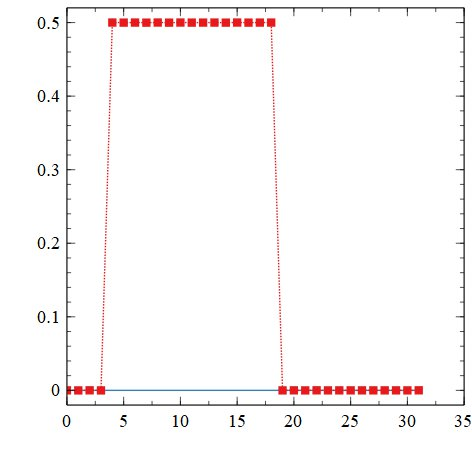
\includegraphics[width=0.5\textwidth]{pulse32}}
    \subfloat[Convoluzione]{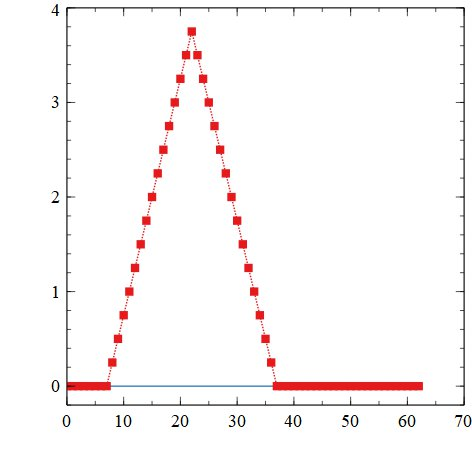
\includegraphics[width=0.5\textwidth]{pulse32conv}}
    \caption{Convoluzione di un impulso rettangolare con sé stesso. In rosso è segnata la parte reale e in blu la parte immaginaria}
    \label{fig:pulse32conv}
\end{figure}

\subsection{GPU}
Per implementare la convoluzione sulla GPU è necessario individuare i thread che è possibile parallelizzare e racchiuderli in uno o più kernel. Nel caso in esame si è deciso di utilizzare l'implementazione che Smith chiama ``algoritmo dal lato dell'uscita'' \cite[pp.~116-121]{dspguide}, il quale differisce dall'algoritmo precedentemente illustrato nell'implementazione sulla CPU per il fatto che si calcolano i contributi di vari campioni dell'ingresso rispetto ad un solo campione in uscita. I due algoritmi, seppur presentino due punti di vista diversi, sono equivalenti e restituiscono lo stesso risultato.

Bisogna prestare attenzione al fatto che dato un kernel di un filtro di $M$ elementi, il valore dell'elemento $i$-esimo dell'uscita è uguale al prodotto dell'elemento $i-j$ esimo dell'ingresso con l'elemento $j$-esimo del kernel del filtro, con $j = 0 ... M-1$.

Il kernel CUDA utilizzato per compiere questa operazione ridotto alle sue operazioni essenziali è il seguente:

\begin{lstlisting}
__global__ void cudaconvolver_kernel(SignalBuffer_t device_buffer, SignalBuffer_t kernel_buffer, SignalBuffer_t out_buffer, size_t channel)
{
    int k = blockIdx.x * blockDim.x + threadIdx.x;
    ...
    cuComplex temp_sample = make_cuComplex(0,0);
    for (int i = 0; i < kernel_size; i++)
    {
        kernel_sample =
            get_sample(kernel_buffer, SIGNAL_CHANNEL, i);
        input_sample =
            get_sample(device_buffer, channel, k-i);
        temp_sample = cuCaddf(temp_sample,
            cuCmulf(kernel_sample, input_sample));
    }
    set_sample(out_buffer, channel, index, temp_sample);
    ...
}
\end{lstlisting}

Si noti la presenza dell'indice $k$, il quale viene calcolato in base agli indici del thread corrente e del blocco corrente; esso identifica la posizione $k$ dell'elemento dell'uscita da calcolare. 

Se il segnale in ingresso è composto di $N$ punti e il kernel del filtro è composto da $M$ punti, il segnale in uscita è di $N+M-1$ punti; infatti la funzione kernel viene eseguita $N+M-1$, ovvero è presente una esecuzione della funzione per ogni elemento in uscita.

Nel codice mostrato è stato tolta la parte per la gestione dell'effetto di ``overlap'' in modo da rendere evidenti le parti fondamentali della sua implementazione per la GPU.

Il grafico in figura \ref{fig:convtime} rappresenta il tempo necessario per compiere una convoluzione utilizzando un kernel di un filtro di dimensioni fisse (128 punti) e facendo variare la lunghezza del file in ingresso da elaborare. Inoltre per quanto riguarda la GPU sono visualizzati anche valori diversi di lunghezza del buffer di elaborazione, in quanto, a differenza della CPU che non risente della grandezza dello stesso, la GPU presenta prestazioni via via migliori all'aumentare della dimensione del buffer, poiché un buffer più grande significa elaborare più dati in parallelo.
\begin{figure}[h]
    \centering
    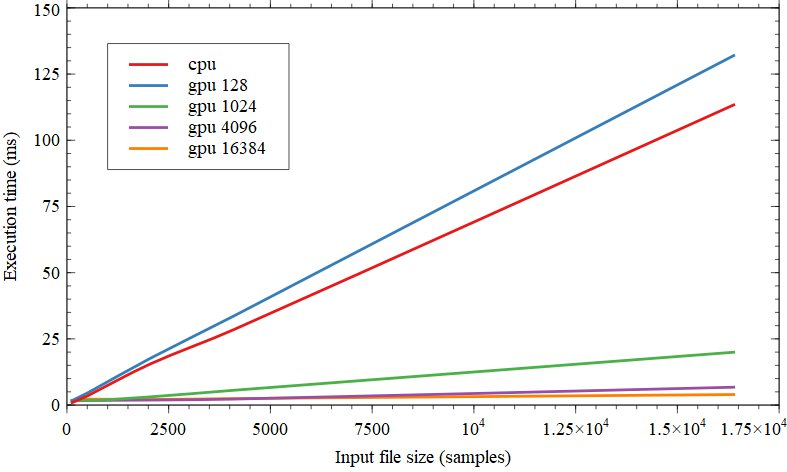
\includegraphics[width=\textwidth]{conv-time}
    \caption{Tempo di convoluzione, CPU e GPU a confronto}
    \label{fig:convtime}
\end{figure}

\section{DFT}
Un secondo algoritmo interessante da implementare è la trasformata di Fourier discreta. Essa trova larga applicazione come strumento di analisi spettrale dei segnali, oltre ad essere un punto di partenza per poi introdurre la \textit{Fast Fourier Transform} (FFT).

Come indicato nell'equazione \ref{eq:dft}, la DFT è sostanzialmente una sommatoria di un prodotto di numeri complessi, notiamo però che a differenza della equazione della convoluzione (\ref{ed:convoluzionediscreta}) il valore massimo della sommatoria dipende dalla lunghezza del segnale. Questo significa che nella implementazione saranno necessari due cicli \lstinline{for} innestati che dipendono entrambi dalla lunghezza del segnale. Tale configurazione di cicli \lstinline{for} restituisce una complessità computazionale di tipo $O(N^2)$. Motivo ulteriore per cui si è sviluppato l'algoritmo della FFT.

\subsection{CPU}
L'implementazione della trasformata di Fourier discreta è ricavata direttamente dalla sua equazione.

\begin{lstlisting}
void dft_wsio(SignalBuffer_t* bufferIn, SignalBuffer_t* bufferOut, size_t channel, size_t size)
{
    ...
    for (size_t k = 0; k < size; k++)
    {
        ...
        for (size_t i = 0; i < size; i++)
        {
            cuComplex s =
                cuComplex_exp(-2 * M_PI * k * i / size);
            cuComplex sample =
                get_sample(*bufferIn, channel, i);
            cuComplex outs =
                get_sample(*bufferOut, channel, k);
            outs = cuCaddf(outs, cuCmulf(sample, s));
            set_sample(*bufferOut, channel, k, outs);
        }
    }
    ...
}
\end{lstlisting}

\lstinline{cuComplex_exp(float x)} è una funzione che restituisce il numero complesso $e^{jx}$. L'algoritmo prende in input un buffer di cui effettuare la trasformata, un buffer in cui inserire il risultato della trasformazione, il canale dei buffer su cui operare e la dimensione in punti della trasformata. Come esposto in precedenza la funzione \lstinline{get_sample} restituisce il numero complesso $0$ nel caso il valore dell'indice sia fuori range. Questo permette di implementare facilmente la dft di un buffer con un pad di zeri alla sua destra.

\begin{figure}[h]
    \centering
    \subfloat[Impulso]{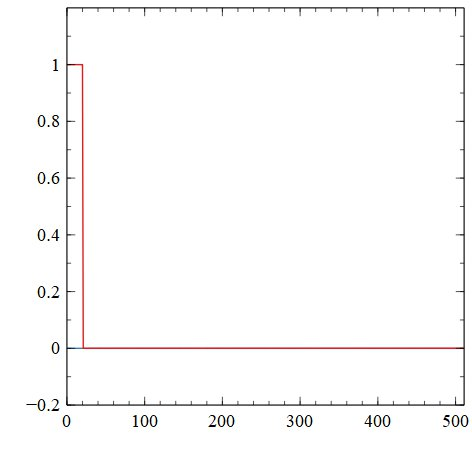
\includegraphics[width=0.5\textwidth]{pulse512}}
    \subfloat[Dft]{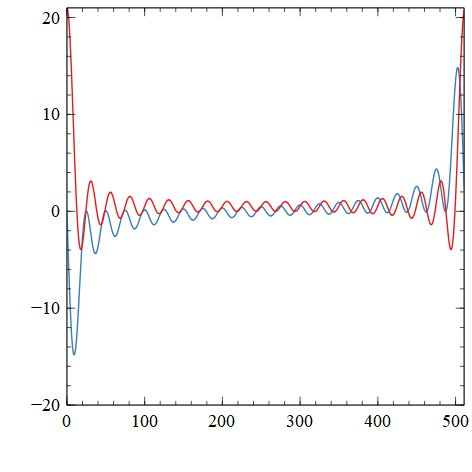
\includegraphics[width=0.5\textwidth]{pulse512dft}}
    \caption{DFT di un impulso di 512 campioni. In rosso è segnata la parte reale e in blu la parte immaginaria}
    \label{fig:pulse512}
\end{figure}

Inserendo nel programma l'impulso di 512 campioni mostrato in figura \ref{fig:pulse512}a si ottiene la trasformata in figura \ref{fig:pulse512}b. Come è facile notare, il segnale di partenza ha solo componente reale, quindi la sua trasformata è simmetrica rispetto a $N/2$ in modo pari per la parte reale e in modo dispari per la parte immaginaria.

\subsection{GPU}
L'operazione di trasformata di Fourier discreta è implementata sulla GPU utilizzando il seguente kernel:

\begin{lstlisting}
__global__ void cudadft_kernel_dft(SignalBuffer_t device_buffer, SignalBuffer_t out_buffer, size_t channel, size_t size)
{
    int k = blockIdx.x * blockDim.x + threadIdx.x;
    ...
    cuComplex temp = make_cuComplex(0, 0);
    for (int i = 0; i < size; i++)
    {
        cuComplex sample =
            get_sample(device_buffer, channel, i);
        cuComplex s
            = cuComplex_exp(-2.0f * PI * k * i / size);
        temp = cuCaddf(temp, cuCmulf(sample, s));
    }
    set_sample(out_buffer, channel, k, temp);
}

\end{lstlisting}

Anche in questo caso, il kernel viene eseguito in parallelo su tutti i campioni del segnale risultando più prestante della rispettiva implementazione sulla CPU. In particolare si può già notare che la complessità di ogni singolo thread si è ridotta a $O(N)$.

[grafici prestazioni]

\section{Fast Fourier Transform}
L'operazione di DFT è onerosa in termini di calcolo in quanto ha complessita $O(N^2)$, per cui si utilizza spesso la Fast Fourier Transform al suo posto (FFT). Uno degli algoritmi più popolari per il calcolo della FFT è quello ideato da Cooley e Tukey nel 1965. Esso fa uso della decomposizione interlacciata e delle somme a ``farfalla''.

[da espandere con più info]

\subsection{CPU}
La FFT è implementata sulla CPU nel seguente modo:

\begin{lstlisting}
    [codice da ridimensionare]
\end{lstlisting}

[da fare].

\subsection{GPU}

[da fare]


\chapter{GPU per DSP}
\section{Un semplice filtro audio su GPU}
\section{Vantaggi del parallelismo}
\section{Elaborazione real time}

\chapter{Conclusioni}
L'elaborazione digitale di segnali è un argomento vastissimo, con varie sfaccettature e varianti: una cosa che funziona molto bene in un caso, potrebbe funzionare molto male in un altro caso e tutto dipende a cosa bisogna applicare tale operazione. Un esempio lampante è il tempo di elaborazione della FFT presentate nell'ultimo capitolo: la CPU ha prestazioni eccezionali per pochi punti, mentre la GPU ha prestazioni incredibili nel caso opposto. Questo non significa che l'utilizzo di una o l'altra piattaforma sia esclusiva, anzi, per come è architetturata ora la tecnologia il caso ottimo è quello di utilizzare entrambi i ``centri di calcolo''.

La sfida rimane quella di modificare gli algoritmi preesistenti in una loro versione che possa essere calcolata in modo parallelo su una GPU. Come si è visto, non sempre è possibile parallelizzare l'intero processo in una volta sola e a volte bisogna scendere a compromessi e utilizzare funzioni di sincronizzazione. 

Nonostante ciò, le prestazioni ottenute dalla GPU sono a dir poco incredibili e soprattutto i grafici presentati mostrano uno \textit{scaling} molto promettente. Non a caso, infatti, questi dispositivi vengono utilizzati per la ricerca nel campo delle intelligenze artificiali e nella costruzione di supercomputer.

\appendix
\chapter{Appendix Title}
\chapter{Funzioni aggiuntive}
\section{Attrezzatura utilizzata}
Il programma che è stato utilizzato nel corso di questa tesi è stato scritto ed eseguito sulla macchina seguente:
\begin{itemize}[nosep]
    \item CPU: Intel Core i5-6500 @3.20GHz, 4 Cores.
    \item RAM: 16GB
    \item GPU: Nvidia GeForce GTX 970
    \begin{itemize}[nosep]
        \item CUDA Driver version: 10.2
        \item CUDA Capability: 5.2
        \item Global Memory: 4096MB
        \item CUDA Cores: 1664
        \item Max clock rate: 1.25GHz
        \item Memory clock rate: 3505Mhz
        \item Memory bus width: 256 bit
        \item Max thread per block: 1024
        \item nvcc version: V10.2.89
    \end{itemize}
\end{itemize}

\section{Codice operazione a ``farfalla''}
\begin{lstlisting}
    void butterfly_calculation(cuComplex* a, cuComplex* b, cuComplex w)
    {
        cuComplex aa = *a;
        cuComplex bw = cuCmulf(*b, w);
    
        *a = cuCaddf(aa, bw);
        *b = cuCsubf(aa, bw);
    }    
\end{lstlisting}

\end{document}